\documentclass[runningheads]{llncs}
\usepackage{graphicx}
\usepackage[T1]{fontenc}
\usepackage[utf8]{vietnam}
\usepackage{listings}
\usepackage{color}

\definecolor{dkgreen}{rgb}{0,0.6,0}
\definecolor{gray}{rgb}{0.5,0.5,0.5}
\definecolor{mauve}{rgb}{0.58,0,0.82}

\lstset{frame=tb,
  language=Python,
  aboveskip=3mm,
  belowskip=3mm,
  showstringspaces=false,
  columns=flexible,
  basicstyle={\small\ttfamily},
  numbers=none,
  numberstyle=\tiny\color{gray},
  keywordstyle=\color{blue},
  commentstyle=\color{dkgreen},
  stringstyle=\color{mauve},
  breaklines=true,
  breakatwhitespace=true,
  tabsize=2
}

\begin{document}
\title{Xử lý và phân loại bình luận tiếng Việt bằng Spark và PyTorch}
\author{Từ Quốc Huy\inst{1} \and Phạm Phong Phú\inst{1} \and Đặng Việt Dũng\inst{1}}	
\authorrunning{Từ Quốc huy \and Phạm Phong Phú \and Đặng Việt Dũng}
\institute{Trường Đại học Công nghệ Thông tin, Đại học Quốc gia Thành phố Hồ Chí Minh
\email{\{huytq.15,phupp.15,dungdd.15\}@grad.uit.edu.vn}}
\maketitle

\begin{abstract}
Các mạng xã hội nơi người dùng có thể đăng tải bình luận sẽ gặp vấn đề nhiều người dùng đăng tải các bình luận tiêu cực và công kích cá nhân. Để xử lý những bình luận này, bao gồm việc ẩn các bình luận tiêu cực và hạn chế các người dùng thường hay đăng các nội dung tiêu cực tốn khá nhiều chi phí và công sức. Vấn đề đặt ra là cần một công cụ có thể nhận diện và tự đông xử lý các bình luận tiêu cực. Hiện nay thì xử lý ngôn ngữ tự nhiên bằng Spark và PyTorch là hai hướng tiếp cận để có thể giải quyết bài toán phân loại bình luận. Sau khi xử lý dữ liệu và huấn luyện mô hình bằng thuận toán Logistic Regression (LR) trên Spark và Recurrent Neural Network (RNN) bằng PyTorch thì kết quả là hai mô hình có độ chính xác tương đương nhau và đủ để sử dụng trong thực tế.

\keywords{Xử lý ngôn ngữ tự nhiên \and Bình luận \and Spark \and PyTorch}
\end{abstract}

\section{Giới thiệu}

Bài toán đặt ra dựa trên tình huống thực tế đối với công việc hàng ngày của một thành viên trong đội ngũ kiểm duyệt bình luận bằng tiếng Việt trên một trang web mạng xã hội. Người sử dụng trang web có thể đăng tải các bình luận, mà nội dung bình luận có thể là nội dung công kích cá nhân hoặc tiêu cực. Để giải quyết vấn đề này thì thường phải có một đội kiểm duyệt nội dung để ẩn các bình luận này. Vấn đề đặt ra là số lượng bình luận cần kiểm duyệt càng ngày càng nhiều hơn. Để giải quyết yêu cầu này thì vấn đề xây dựng một hệ thống tự động kiểm duyệt bình luận được đặt ra. Hệ thống tự dộng kiểm duyệt ngoài hỗ trợ vận hành hệ thống hiện tại thì có thể áp dụng cho các bài toán ví dụ như kiểm duyệt cho hệ thống thời gian thực trong tương lai. Tóm lại là cần có một giải pháp kiểm duyệt bình luận dựa trên lịch sử kiểm duyệt sẵn có.

Từ dữ liệu lịch sử kiểm duyệt, có thể thu thập được một bộ dữ liệu gồm nội dung bình luận và trạng thái kiểm duyệt. Dữ liệu gồm 1 triệu dòng được trích xuất trong 6 tháng đầu năm 2021.

\begin{figure}
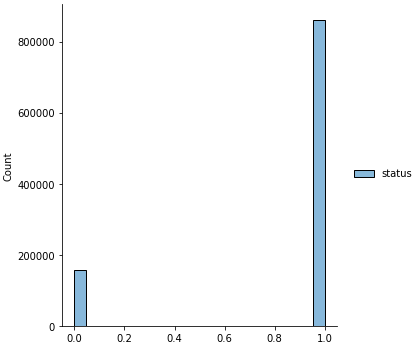
\includegraphics[scale=0.7]{sns.png}
\centering
\caption{Phân phố trạng thái trên tập bình luận \label{figSeaborn}}
\end{figure}

\section{Xử lý dữ liệu}

\subsection{Tiền xử lý dữ liệu}

Dữ liệu đầu vào là các bình luận bằng tiếng Việt. Các bình luận này do người dùng nhập nên tiềm ẩn một số vấn đề như từ viết tắt, viết sai chính tả, chứa email, hashtag, các emoji,... Để có thể phân tích dữ liệu, cần làm sạch dữ liệu đầu vào.

\paragraph{Loại bỏ Hashtag} bỏ kí tự \# trong \#hashtag để đưa về dạng chuỗi không có kí tự \#
\paragraph{Loại bỏ URL} bỏ các chuỗi được nhận diện là URL
\paragraph{Loại bỏ email} bỏ các chuỗi nhận diện là email
\paragraph{Unescape các kí tự trong URL} phải unescape các kí tự đặc biệt nếu dữ liệu là dạng HTML hoặc XML
\paragraph{Loại bỏ các kí tự không phải chữ} chỉ giữ lại các kí tự a-z và A-Z, đồng thời các kí tự có dấu tiếng Việt.
\paragraph{Loại bỏ các chữ mà người dùng nhập đúp} loại bỏ các chữ người dùng nhập đúp, ví dụ người dùng có thể nhập "anhhh", trong khi đúng thì phải là "anh", trường hợp này phải bỏ đi cụm "hh".
\paragraph{Đồng bộ một số từ} đưa một số từ đồng nghĩa về đòng dạng, ví dụ từ "haha" sẽ được dùng chung cho tiếng cười, mà người dùng có thể nhập là "hahaha", "hoho", "hihi", "kkk",...

\begin{lstlisting}
df
  .withColumn("content", regexp_replace(col("content"), hashtag\_regex, "$1"))
  .withColumn("content", regexp_replace(col("content"), url\_regex, ""))
  .withColumn("content", regexp_replace(col("content"), email\_regex, ""))
  .withColumn("content", html_unescape("content"))
  .withColumn("content", regexp_replace(col("content"), not\_char\_regex, " "))
  .withColumn("content", regexp_replace(col("content"), r"([^oplen])\1+", "$1"))
  .withColumn("content", regexp_replace(col("content"), r"([oplen])\1\1+", "$1"))
  .withColumn("content", trim(col("content")))
\end{lstlisting}

\subsection{Huẩn luyện mô hình bằng Logistic Regression trong Spark}

\subsubsection{Chuẩn bị dữ liệu}

\subsubsection{Xây dựng mô hình}

\subsubsection{Huấn luyện mô hình}

\subsection{Huấn luyện mô hình bằng Recurrent Neural Network trong PyTorch}

\subsubsection{Chuẩn bị dữ liệu}

Một trong những khái niệm chính của TorchText là Field. Chúng xác định cách dữ liệu sẽ được xử lý. Trong phần phân loại bình luận này thì dữ liệu bao gồm cả chuỗi thô của bình luận và trạng thái, "duyệt" hoặc "ẩn".

Các tham số của một Field chỉ định cách dữ liệu sẽ được xử lý. Field TEXT sẽ được sử dụng để xác định cách bình luận sẽ được đánh giá và Field LABEL để xử lý trạng thái bình luận.

\paragraph{Field TEXT:}ta có tham số tokenize="spacy". Điều này xác định rằng "tokenization" (hành động tách chuỗi thành các "token" rời rạc) được thực hiện bằng cách sử dụng trình mã hóa spaCy. Nếu không có đối số mã hóa nào được truyền, thì mặc định chỉ đơn giản là tách chuỗi trên khoảng trắng. Cần chỉ định tokenizer\_language="vi\_core\_news\_lg" để cho TorchText biết mô hình spaCy xử lý tiếng Việt sẽ sử dụng.

\paragraph{Field LABEL} được định nghĩa bởi một LabelField, một lớp con của lớp Field được sử dụng để xử lý các nhãn.

\begin{lstlisting}
CONTENT = data.Field(tokenize = 'spacy',
                  tokenizer_language = 'vi_core_news_lg')
STATUS = data.LabelField(dtype = torch.float)
fields = [('content', CONTENT), ('status', STATUS)]
train_data, valid_data, test_data = data.TabularDataset.splits(
                                        path = './input',
                                        train = 'train_filtered.csv',
                                        validation = 'validation_filtered.csv',
                                        test = 'test_filtered.csv',
                                        format = 'csv',
                                        fields = fields,
                                        skip_header = True
)
\end{lstlisting}

Dữ liệu được đặt trong 3 tập tin, các dữ liệu đều đã được làm sạch từ phần trước.

\begin{figure}
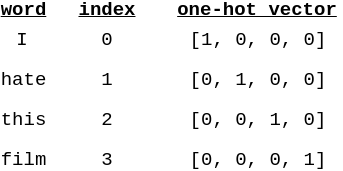
\includegraphics[scale=0.5]{sentiment5.png}
\centering
\caption{Ví dụ one-hot vector \label{figOnehotVector}}
\end{figure}

Tiếp theo là bước xây dựng bộ từ vựng (vocabulary). Các từ vựng được sắp xếp theo thứ tự giảm dần của tần suất xuất hiện và được đại diện bằng một chỉ số. Mỗi chỉ số sẽ được dùng để dựng one-hot vector (Xem hình ~\ref{figOnehotVector}). One-hot vector này là một vector có số chiều bằng số từ trong bộ từ vựng và với từ tương ứng chỉ só thì chiều chỉ số bằng 1, còn lại sẽ bằng 0. Do số lượng của bộ từ vựng quá lớn nên chỉ chọn giữ lại 25.000 từ vựng đầu tiên theo thứ tự giảm dần của độ phổ biến. Đối với những từ đã bị cắt đi thì sẽ được đánh dấu bằng kí tự <unk>. Kích thước của bộ từ vựng sẽ là 25.002, trong đó gồm 25.000 từ phổ biến nhất và hai từ <pad> và <unk>.

\begin{lstlisting}
MAX_VOCAB_SIZE = 25_000
CONTENT.build_vocab(train_data, max_size = MAX_VOCAB_SIZE)
STATUS.build_vocab(train_data)
\end{lstlisting}

Bước cuối cùng của việc chuẩn bị dữ liệu là tạo các iterator. Cần phải duyệt nhiều lần qua iterator trong vòng lặp huấn luyện/đánh giá và chúng trả về một loạt các mẫu (được lập chỉ mục và chuyển đổi thành tensor) ở mỗi lần lặp.

Sử dụng BucketIterator là một loại iterator đặc biệt sẽ trả về một loạt các mẫu trong đó mỗi mẫu có độ dài tương tự nhau, giảm thiểu số lượng <pad> của mỗi mẫu.

\begin{lstlisting}
train_iterator, valid_iterator, test_iterator = data.BucketIterator.splits(
    (train_data, valid_data, test_data), 
    batch_size = 64,
    sort_key = lambda x: len(x.content),
    sort_within_batch = False,
    device = device)
\end{lstlisting}

\subsubsection{Xây dựng mô hình}

Lớp mô hình RNN được tạo ra trong PyTorch là một lớp con của nn.Module. 

\begin{lstlisting}
class RNN(nn.Module):
    def __init__(self, input_dim, embedding_dim, hidden_dim, output_dim):        
        super().__init__()        
        self.embedding = nn.Embedding(input_dim, embedding_dim)        
        self.rnn = nn.RNN(embedding_dim, hidden_dim)        
        self.fc = nn.Linear(hidden_dim, output_dim)        
    def forward(self, text):        
        embedded = self.embedding(text)        
        output, hidden = self.rnn(embedded)
        assert torch.equal(output[-1,:,:], hidden.squeeze(0))        
        return self.fc(hidden.squeeze(0))
\end{lstlisting}

\begin{figure}
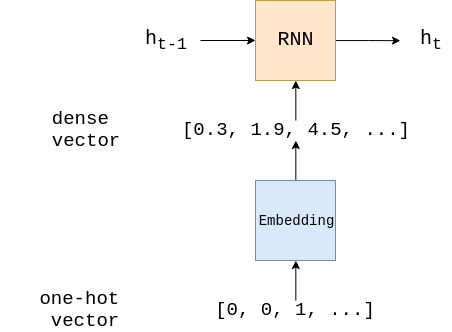
\includegraphics[scale=0.5]{sentiment7.png}
\centering
\caption{Mô tả quá trình chuyển từ one-hot vector thành dense vector \label{figOnehotToDense}}
\end{figure}

\paragraph{Hàm \_\_init\_\_} thì phải định nghĩa các tầng embedding, RNN và linear. Đa số các tầng sẽ có các tham só mặc định trừ một số trường hợp đặc biệt.
Tầng embedding được dùng để chuyển one-hot vector thành một dense embedding vector (Xem hình ~\ref{figOnehotToDense}). Tầng embedding này chỉ đơn giản là một tầng kết nối đầy đủ. Ngoài việc giảm số chiều của đầu vào cho RNN, các từ có tác động tương tự đến cảm xúc của bài đánh giá cũng được ánh xạ gần nhau trong không gian vector dày đặc này. 
Tầng RNN sẽ nhận dense vector và trạng thái ẩn \textit{$h_{t-1}$} để tính ra trạng thái ẩn \textit{$h_{t}$}. Cuối cùng tầng linear lấy trạng thái ẩn cuối cùng và đăng trạng thái này vào tầng kết nối đầy đủ \textit{$f(h_T)$}, và chuyển nó thành chiều đầu ra tương ứng.

\paragraph{Hàm forward} được gọi khi đăng các mẫu vào mô hình.

\subsubsection{Huấn luyện mô hình}

Đầu tiên phải tạo một optimizer. Optimizer được dùng để cập nhật các tham số cho mô hình. Thuật toán stochastic gradient descent (SGD) sẽ được sử dụng.
Tiếp theo phải định nghĩa loss function, hay được gọi là criterion trong PyTorch.
Cần phải huấn luyện mô hình qua nhiều lần lặp. Mỗi lần lặp thì mô hình sẽ tính lại và chọn ra mô hình cho độ mất mát trên tập validate tốt nhất.

\section{Kết quả}

\subsection{Mô hình bằng Logistic Regression trong Spark}

Mô hình LR đạt độ chính xác 87.3\% trên tập validation và đạt 87.2\% trên tập test.

\begin{lstlisting}
Validation accuracy: 87.31911%
Test accuracy: 87.18459%
\end{lstlisting}

\subsection{Mô hình bằng Recurrent Neural Network trong PyTorch}

Sau 5 lần huấn luyện thì mô hình RNN đạt độ chính xác 87.6\% trên tập validation và đạt 85.9\% trên tập test.

\begin{lstlisting}
Validation accuracy: 87.61%
Test accuracy: 85.91%
\end{lstlisting}

\section{Kết luận}

\end{document}
